\documentclass[border=2pt]{standalone}

\usepackage{tikz}
\usetikzlibrary{positioning,decorations.pathreplacing,fit}
\usetikzlibrary{decorations.markings,arrows.meta,shapes.arrows,arrows}
\usetikzlibrary{calc}

\definecolor{darkgreen}{RGB}{0,128,80}


\begin{document}


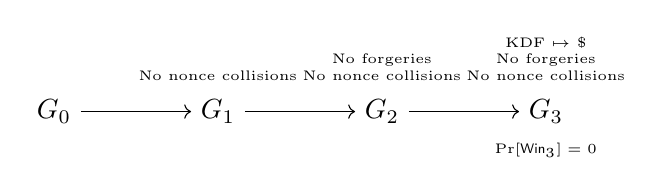
\begin{tikzpicture}[
	arrow double line/.style={
		double distance = 20pt,
   		shorten <= 11, 	
   		shorten >= 16,
   		very thick,
	    postaction = {
    		draw = white,
	 	    line width = 20pt,
	 	    shorten <=-.1pt,
	 	    shorten >=-.1pt,	
	    },
	    postaction = {
	    	decorate, 
	    	decoration = {
	    		markings, 
	    		mark=at position 0 with {
	    			\arrow[xshift=26.6pt]{Straight Barb[reversed,length=-1pt 0.7]}
	    		},
	    		mark = at position 1 with {
   	    			\arrow[xshift=10.6pt]{Straight Barb[length=-1pt 0.7]}
   	    		}
	    	}
	    }
	},
	mysingle/.style = {
		double distance = 22,
		shorten <= 10.5, 	
		shorten >= 14,
		very thick,
		postaction = {
	 		draw = white,
			line width = 22pt,
			shorten <=8pt,
			shorten >=-.5pt,	
		},
		postaction = {
			decorate, 
			decoration = {
				markings, 
				mark = at position 1 with {
					\arrow [xshift=15]{Straight Barb[length=15]}
				}
			}
		},	
	},	
	mybrace/.style= {
		decorate, decoration={brace,amplitude=5pt,raise=5pt}, thick
	},
	]

	\def\InterGameSpace{1.4}
	
	

	\node (G0) {$G_0$};
	\node[right = \InterGameSpace of G0] (G1) {$G_1$};
	\node[right = \InterGameSpace of G1] (G2) {$G_2$};
	\node[right = \InterGameSpace of G2] (G3) {$G_3$};
	
	\draw[->] (G0) -- (G1);
	\draw[->] (G1) -- (G2);
	\draw[->] (G2) -- (G3);


	\uncover<3->{ \node[above = 0 of G1,align=center,font=\tiny] () {\phantom{KDF $\mapsto$ $\$$}\\\phantom{No forgeries}\\No nonce collisions}; }
	\uncover<5->{ \node[above = 0 of G2,align=center,font=\tiny] () {\phantom{KDF $\mapsto$ $\$$}\\No forgeries\\No nonce collisions}; }
	\uncover<7->{ \node[above = 0 of G3,align=center,font=\tiny] () {KDF $\mapsto$ $\$$\\No forgeries\\No nonce collisions}; }
	
%	\draw[bend right] (G0.south east) to node [auto,below,font=\tiny] {$\Pr[]$} (G1.south west);

%	\node[below = 0 of G0,font=\tiny] () {$\Pr[\mathsf{Win}] = ?$};
 
 	\uncover<9->{
 		\node[below = 0 of G3,font=\tiny,align=center] () {$\Pr[\mathsf{Win}_3] = 0$};
 	}
\end{tikzpicture}



\end{document}